\documentclass[conference]{IEEEtran}
\usepackage{graphicx}
\usepackage[strings]{underscore}
\usepackage{biblatex}

%Title
\title{Alternative Edge Detection Methods}
\author{
    \IEEEauthorblockN{Sotheanith Sok}
    \IEEEauthorblockA{
        Department of Engineering\\ 
        California State University of Long Beach\\
        Sotheanith.Sok@student.csulb.edu
    }
}
\date{September 26 2021}

\addbibresource {refs.bib}

\begin{document}
\maketitle

\section{Introduction}
In general, an image can be manipulated by convolving it with various kernels. From noise minimizing with Gaussian filter to edge detection with Prewitt filter, information can be added, removed, or extracted from an image through the use of specific filter. Thus, selecting a correct filter is a crucial step in performing a proper manipulation of an image. As such, this paper will explore four popular edge detection methods: Roberts Cross, Canny Edge Detector, Difference of Gaussian, and Laplacian of Gaussian including their functionalities, their advantages, and their limitations.  

\section{Roberts Cross}
In computer vision, Roberts Cross is a filter for detecting edges in a grayscale image. It works by examining gradient magnitude among adjacent and diagonal pixels which is a strong indication of edges. The gradient magnitude can be calculated from points convolved from two special kernels.
\begin{figure}[!htb]
    \centering
    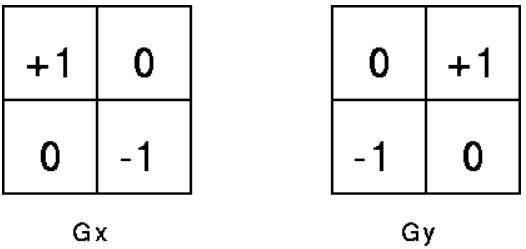
\includegraphics[scale = 0.3]{RC_K.png}
    \caption{Roberts Cross Kernels \cite{fisher-perkins-walker-wolfart:2003}.}
\end{figure}
Each kernel is tasked with detecting 45° edges in its respective orientation and the resulting convolved matrices represent the two components of the gradient magnitude. According to \cite{fisher-perkins-walker-wolfart:2003}, the gradient magnitude and direction can be represented as \[|G| = \sqrt{Gx^2+Gy^2}\] \[\theta = atan2(Gy,Gx)\] where:
\begin{description}
    \item[$|G|$] is the gradient magnitude.
    \item[$\theta$] is the gradient direction.
    \item[$Gx$] is the first gradient component.
    \item[$Gy$] is the second gradient component.
\end{description}
Additionally, since the gradient magnitude is always positive and its actual magnitude does not affect the algorithm, the gradient magnitude formula can be approximate as \cite{fisher-perkins-walker-wolfart:2003} \[|G| = |Gx| + |Gy|\]. In practice, however, it is common to approximate gradient magnitude in a single pass with the following formula \cite{fisher-perkins-walker-wolfart:2003} \[|G| = |P1-P4| + |P2-P3|\].
\begin{figure}[!htb]
    \centering
    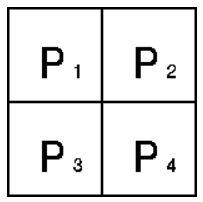
\includegraphics[scale = 0.3]{RC_AK.PNG}
    \caption{Robert Cross kernal for approximate gradient magnitude in a single pass \cite{fisher-perkins-walker-wolfart:2003}.}
\end{figure}

\section{Canny Edge Detector}
Canny Edge Detector is a multi-stage algorithm for detecting edges in a grayscale image. It is composed of five stages: noise reduction, gradient calculation, non-maximum suppression, double threshold, and edge tracking with hysteresis.

As with most first derivative edge detection algorithms, Canny Edge Detector is sensitive to noises. As the result, the first step is noise minimization of an image through the use of blurring filters such as a mean filter, an average filter, or a Gaussian filter.

Once completed, the algorithm will utilize either a Prewitt filter, specialize in detecting edges in a horizontal or a vertical direction, or a Roberts Cross filter, specialize in detecting edges in diagonal directions, to generate the magnitude and the direction of the gradient with the following approximation formulas \cite{sofiane-sahir:2019} \[|G|=|Gx|+|Gy|\] \[\theta = atan2(Gy,Gx)\]. Since each pixel can only have up to eight neighbors, the gradient direction will be round to one of the four directions: 0°, 45°, 90° and 135°.

Next, the algorithm will perform a non-maximum suppression on each pixel using its gradient magnitude and its gradient direction. During this stage, each pixel will have its gradient magnitude compare to its neighbors that exist along the pixel's direction. For example, if a pixel has a gradient direction of 45°, then its comparable neighbors are the top-right pixel and the bottom-left pixel. If a pixel has the highest gradient magnitude when compared to its comparable neighbors, the pixel's gradient magnitude is preserved. On the contrary, if a pixel does not have the highest gradient magnitude when compared to its comparable neighbors, the pixel's gradient magnitude will be set to 0.
\begin{figure}[!htb]
    \centering
    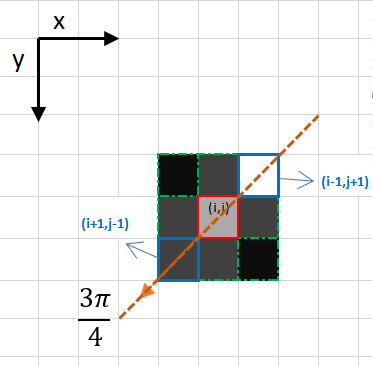
\includegraphics[scale = 0.3]{CED_nms.png}
    \caption{Non-maximum suppression on the pixel i, j with $\theta$ = 45° \cite{sofiane-sahir:2019}.}
\end{figure}

The following stage after the non-maximum suppression stage is the double threshold stage. In this phase, all pixels will be classified into three categories: strong, weak, and irrelevant using two thresholds: high and low. If a pixel has a gradient magnitude greater than the high threshold, it will be classified as a strong pixel. In contrast, if a pixel has a gradient magnitude between the high threshold and the low threshold, it will be classified as a weak pixel. As for the remaining pixels, they will be classified as an irrelevant pixel.

The final stage of Canny Edge Detector is edge tracking with hysteresis. For this stage, all weak pixels will reclassify as either a strong pixel or an irrelevant pixel. If a weak pixel has at least one of its neighbors as a strong pixel, it will be reclassified as a strong pixel. For other pixels that do not have a strong pixel as their neighbors, it will be reclassified as an irrelevant pixel.
\begin{figure}[!htb]
    \centering
    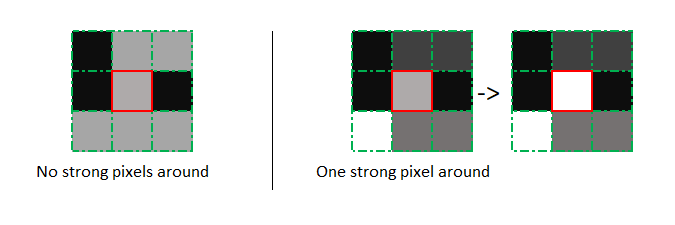
\includegraphics[scale = 0.3]{CED_hysteresis.png}
    \caption{The two cases for edge tracking with hysteresis \cite{sofiane-sahir:2019}.}
\end{figure}

\section{Difference of Gaussian}
Difference of Gaussian is a feature enhancement algorithm that takes advantage of two blurred images convolved from two different Gaussian kernels. The algorithm starts by generating two different Gaussian kernels with the following formula \cite{fisher-perkins-walker-wolfart-2:2003} \[G(x,y,\sigma)=\frac{1}{2\pi\sigma^2}e^{-\frac{x^2+y^2}{2\sigma^2}}\] where:
\begin{description}
    \item[$G$] is the Gaussian.
    \item[$x$] is the first gradient component.
    \item[$y$] is the second gradient component.
    \item[$\sigma$] is the standard deviation.
\end{description}
. Afterwards, the original image will be convolved by the two Gaussian kernels to create two convolved images and the difference between the two convolved images will be use to determine pixel's frequency. Any pixel with intensity difference closer to 0 indicates a low-frequency or non-edges area and any pixel with intensity difference significantly larger than 0 indicates a high-frequency or edges area.

\begin{figure}[!htb]
    \centering
    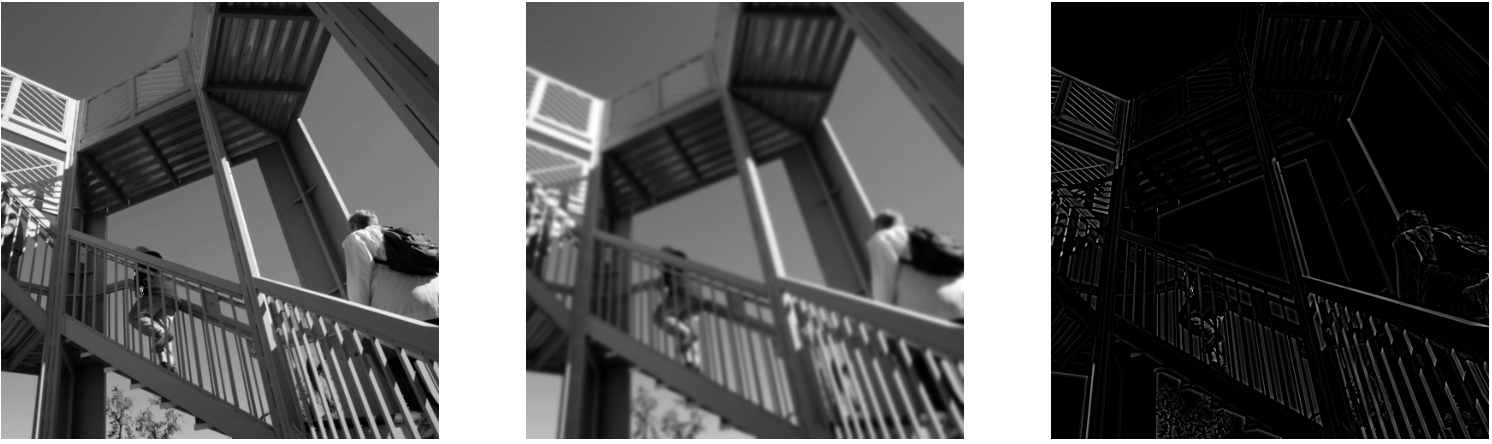
\includegraphics[width=\linewidth,scale = 0.3]{DoG.png}
    \caption{The difference of Gaussian between $\sigma$ = 0.5 and $\sigma$ = 2 \cite{scipy-examples:2021}.}
\end{figure}

It should be noted that pixel intensity difference can also be a negative number. Such a scenario can be handle in two ways: set all negative numbers to 0 or scale the entire image such that its starting value is 0. Last but not least, Difference of Gaussian can also be referred to as a band-pass filter since it suppresses high-frequency spatial information with Gaussian blurring and low-frequency spatial information with subtraction.

\section{Laplacian of Gaussian}
Laplacian of Gaussian is a second derivative filter for detecting edges. Unlike first derivative filters which rely on local maximum to detect edges, Laplacian of Gaussian relies on zero-crossing where a gradient magnitude of the second derivative cross 0.
\begin{figure}[!htb]
    \centering
    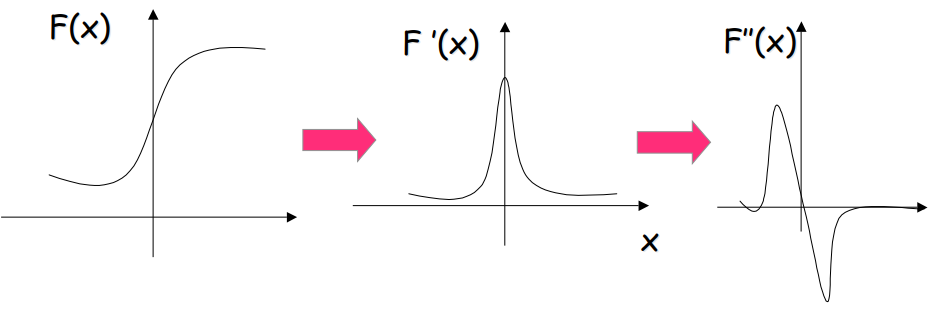
\includegraphics[width=\linewidth,scale = 0.3]{LoG_derrivatives.PNG}
    \caption{Graphs of a pixel's intensity, its first derrivative, and its second derrivative \cite{collins:2007}.}
\end{figure}
The Laplacian of Gaussian kernel can be calculated with the following formula\cite{parikh:2020} \[LoG(x,y,\sigma)=-\frac{1}{\pi\sigma^4}\left[1-\frac{x^2+y^2}{2\sigma^2}\right]e^{-\frac{x^2+y^2}{2\sigma^2}}\] where:
\begin{description}
    \item[$LoG$] is the Laplacian of Gaussian.
    \item[$x$] is the first gradient component.
    \item[$y$] is the second gradient component.
    \item[$\sigma$] is the standard deviation.
\end{description}

This approach of finding edges has its advantage and disadvantage. For the advantage, Laplacian of Gaussian tends to perform better than first derivative filters at finding edges since it is hypersensitive to a spike in pixel's intensity. However, due to its sensitivity, Laplacian of Gaussian also performs poorly on images with a lot of noise. Thus, it is recommended that any image should have its noise minimize before being process by this filter.

\section{Final Thought}
Roberts Cross, Canny Edge Detector, Difference of Gaussian, and Laplacian of Gaussian are methods that designed to detect edges in a grayscale image. While all of them perform well in various circumstances, none of them is a universally correct choice. As such, it is important that one should examine the datasets and pick a method that performs well under the given contrains.

\printbibliography

\end{document}
